\documentclass[a4paper,12pt]{article}
\usepackage[utf8] {inputenc}
\usepackage[russian] {babel}
\usepackage{amssymb}
\usepackage{amsthm}
\usepackage{array}
\usepackage{amsmath}
\usepackage{amsfonts}
\usepackage{graphicx}
\graphicspath{{pics/}}
\usepackage{changepage}
\usepackage{enumitem}
\usepackage[nottoc,numbib]{tocbibind}
\usepackage{subcaption}

\usepackage{wrapfig}
\newtheorem{defi} {Определение}
\newtheorem{theorem} {\bf Теорема}
\theoremstyle{remark}
\newtheorem{remark} {Замечание}

\usepackage{geometry} % Меняем поля страницы
\geometry{left=0.5cm}% левое поле
\geometry{right=0.5cm}% правое поле
\geometry{top=1cm}% верхнее поле
\geometry{bottom=2cm}% нижнее поле

\begin{document}
	
	\begin{titlepage}
		\begin{center}
			\large
			ФЕДЕРАЛЬНОЕ ГОСУДАРСТВЕННОЕ БЮДЖЕТНОЕ ОБРАЗОВАТЕЛЬНОЕ\\УЧРЕЖДЕНИЕ ВЫСШЕГО ОБРАЗОВАНИЯ\\«МОСКОВСКИЙ ГОСУДАРСТВЕННЫЙ УНИВЕРСИТЕТ\\имени М. В. ЛОМОНОСОВА»
			
			\vspace{0.8 cm}
			МЕХАНИКО-МАТЕМАТИЧЕСКИЙ ФАКУЛЬТЕТ
			
			\vspace{0.8 cm}
			КАФЕДРА теории пластичности
			
			\vspace{2.4 cm}
			ВЫПУСКНАЯ КВАЛИФИКАЦИОННАЯ РАБОТА\\(ДИПЛОМНАЯ РАБОТА)\\специалиста
			
			\vspace{0.8 cm}
			\textbf{ПРИМЕНЕНИЕ МЕТОДОВ АНАЛИЗА БОЛЬШИХ ДАННЫХ ДЛЯ ОЦЕНКИ ВЕЛИЧИНЫ И МЕСТОНАХОЖДЕНИЯ ПОВРЕЖДЕНИЯ В КОНСТРУКЦИИ}
		\end{center}
	
		\vspace{1.6 cm}
		\begin{adjustwidth}{10 cm}{0 cm}
			Выполнил студент\\625 группы\\Мищенко Александр Дмитриевич
			\vspace{1.6 cm}
			\newline
			\underline{ \hspace{6.4 cm}}\\
			подпись студента\\\\
			Научный руководитель:
			профессор Шешенин\\Сергей Владимирович
			\vspace{0.4 cm}
			\newline
			\underline{ \hspace{6.4 cm}}\\
			подпись научного руководителя
		\end{adjustwidth}

		\vspace*{\fill}
		\begin{center}
			Москва\\2018 год
		\end{center}
	\end{titlepage}

	\newgeometry{left=2cm, top=1cm, bottom=2cm, right=1cm}
	\tableofcontents
	
	\newpage
	\section{Введение}
	Дефекты в конструкциях являются причиной аварий и в то же время неизбежно возникают в процессе эксплуатации. Множество работ последних десятилетий было посвящено методологиям обнаружения дефектов на ранней стадии. Они позволяют проводить своевременную замену деталей конструкций без неприятных последствий. Сбор данных о состоянии конструкций и алгоритмы для обработки этих данных в совокупности носят название Structural Health Monitoring (SHM).
	
	Задачи SHM принято разделять на четыре последовательные ступени  \cite{review}:
	\begin{enumerate}[itemsep=0cm, topsep=0.2cm]
		\item Определение наличия повреждения в конструкции.
		\item Определение местонахождения повреждения в конструкции.
		\item Оценка величины повреждения.
		\item Прогнозирование оставшегося срока службы конструкции.
	\end{enumerate}
	
	Эта работа сосредоточена на втором и третьем пунктах и затрагивает первый: они носят общее название \textit{идентификации дефектов}. Последний пункт относится к так называемым задачам оценки ресурса конструкции и анализа усталостной долговечности.
	
	Для идентификации дефектов применяются \textit{недеструктивные методы}. Они позволяют определять параметры дефектов с минимально возможным вмешательством в исследуемый объект. Примеры недеструктивных методов \cite{damage_identification_beam_crossectional_area}:
	\begin{itemize}[itemsep=0cm, topsep=0.2cm]
		\item Визуальный осмотр -- невооружённым глазом или с помощью оптических приборов.
		\item Капиллярный контроль -- полости поверхностных трещин заполняют специальными индикаторными веществами (пенетрантами), проникающими в трещины под действием сил капиллярности и повышающими контрастность дефектных участков.
		\item Магнитно-порошковая дефектоскопия. Принцип действия основан на создании поля рассеяния над дефектами детали с последующим выявлением их магнитной суспензией.
		\item Радиография -- облучение ренгеновскими, $\alpha$-, $\beta$-,  $\gamma$- лучами и нейтронами в расчете на то, что трещины, раковины или включения инородного материала ослабляют лучи.
		\item Ультразвуковая дефектоскопия. Принцип действия основан на свойстве ультразвуковых колебаний отражаться от внутренних дефектов материала, проводящего эти колебания.
	\end{itemize}
	Однако перечисленные ``ручные'' методы не могут быть отнесены к SHM, поскольку не могут применяться автоматически без участия человека. Кроме того, в некоторых случаях они бесполезны: например, когда стоит задача мониторинга состояния мостов и других конструкций огромного размера.
	
	Недеструктивные методы SHM заключаются в применении различных алгоритмов для решения \textit{обратной задачи}. Разделение задач на прямые и обратные формулируется так \cite{crack_detection}: прямая задача состоит в том, чтобы выяснить, как различные заданные повреждения влияют на параметры системы; тогда как обратная задача -- более реалистичная -- измерить параметры системы и по ним предсказать наличие повреждения и его свойства. Таким образом, недеструктивными методами SHM являются разные способы измерения параметров системы и их последующей обработки. Способы измерения могут быть разделены по типу задачи:
	\begin{itemize}[itemsep=0cm, topsep=0.2cm]
		\item Статическая задача -- измерение деформации или сдвигов разных частей конструкции под нагрузкой \cite{artificial_neural_networks_in_damage_detection}, \cite{randomized_trained_neural_networks}.
		\item Динамическая задача -- измерение собственных частот и/или нахождение форм колебаний при этих частотах. \cite{damage_identification_beam_crossectional_area}, \cite{crack_detection}, \cite{multi_stage_neural_networks}.
	\end{itemize}
	В этой работе применяется первый способ.
	
	В качестве испытательного образца рассматривается  консольная балка со скрытым дефектом, имеющим вид расслоения -- распространенного дефекта слоистых композитов. Свободный конец балки нагружается известной силой $F$. Снимаются показания тензодатчиков, расположенных на верхней грани балки. Тензодатчики показывают перемещения точек балки вдоль оси, возникающие вследствие деформации. Наличие, величина и местонахождение повреждения влияют на полученные данные, а значит возможно создание алгоритма, решающего обратную задачу. Вместо реальных экспериментов с балками были созданы их конечно-элементные модели в программном пакете Wolfram Mathematica.
	
	Балки используются в качестве образцов в большинстве рассмотренных автором статей, поскольку они просты в изучении, и в то же время успешная проверка алгоритмов на их примере открывает путь к пониманию поведения более сложных конструкций \cite{crack_detection}.
	
	Рассматривается \textit{задача классификации}, то есть на выходе алгоритм выдает распределение вероятностей местонахождения/величины дефекта из набора дискретных значений. В качестве метода решения задачи было выбрано \textit{обучение с учителем} -- один из методов машинного обучения, при котором алгоритм обучается по достаточно большому набору пар «стимул-реакция», которые называются \textit{обучающей выборкой}. Обучающая выборка программно генерируется для каждой задачи из 10 000 экспериментов со случайно выбранными параметрами повреждения. В качестве обучающегося на этих данных алгоритма используется \textit{искусственная нейронная сеть} (ИНС).
	
	ИНС являются одним из классов систем \textit{анализа больших данных} -- компьютерной дисциплины, фокусирующейся на обработке больших объемов ``сырых'' данных, то есть непригодных для человеческого восприятия в исходном виде. В этих данных требуется обнаружить с помощью алгоритмов некие закономерности, или \textit{паттерны}, на основе которых можно, например, научиться делать предсказания для новых данных. В данном случае паттерном служит взаимосвязь между параметрами системы и местонахождением и величиной дефекта. Примеры других классов систем:
	\begin{itemize}[itemsep=0cm, topsep=0.2cm]
		\item Деревья решений -- классификация при помощи деревьев, узлы которых содержат либо значения целевой функции (``листья''), либо атрибуты, по которым различаются случаи. Для классификации нового случая надо спуститься по дереву до одного из листьев.
		\item Эволюционное программирование -- процесс построения программ, организованный как эволюция в мире программ: система вносит в свои дочерние программы модификации и отбирает те из них, которые являются наиболее точными.
		\item Кластерный анализ -- процедура упорядочивания многомерных объектов в сравнительно однородные группы. Относится к задачам обучения без учителя.
	\end{itemize}
	
	Использование ИНС для идентификации дефектов описано в \cite{artificial_neural_networks_in_damage_detection}, \cite{randomized_trained_neural_networks}, \cite{multi_stage_neural_networks}. В работе \cite{artificial_neural_networks_in_damage_detection} ИНС применются для нахождения местоположения и величины повреждения в Т-образном полимерном композите. Предсказания двух независимо обученных ИНС обрабатываются затем третьей, глобальной ИНС. В \cite{randomized_trained_neural_networks} ставится задача идентификации дефектов в консольной балке, однако дефект моделируется домножением матрицы жесткости конечных элементов на заданный коэффициент. Проверяется способность ИНС к обучению отдельно на перемещениях и деформациях модели. Наконец, в \cite{multi_stage_neural_networks} ставится динамическая задача для балки со свободными концами; дефект моделируется домножением модулей Юнга отдельных участков балки на заданные коэффициенты. Используется система из целого дерева нейронных сетей, на вход системы подаются формы колебаний и собственные частоты балки. Стоит отметить, что архитектура ИНС определяется множеством параметров, которые подбираются отдельно для каждой задачи, и зависят во многом от особенностей обучающей выборки. Подробнее об этом в разделе \ref{sec:solving_problem}.
	
	Для написания программ в этой работе использовались языки Wolfram с пакетом NDSolve`FEM` и Python 3.6.4 с open-source библиотеками NumPy, MatPlotLib, TensorFlow, Keras.
	
	\newpage
	\section{Постановка задачи}
	\label{sec:formulation_problem}
	
	Рассматривается консольная балка с жестко зафиксированным левым концом (условие Дирихле) и нагруженная силой $F$ на правом конце (условие Неймана).

	Дефект моделируется полостью в виде эллипса (Рис. \ref{fig:beam_sample}). В качестве входных данных алгоритма используются показания 11 тензодатчиков, расположенных на верхней грани балки. Будем считать, что тензодатчики показывают относительное удлинение, поэтому их показания можно моделировать, просто получая главную компоненту $\varepsilon_{11}$ тензора деформаций. Модуль Юнга взят равным $E = 12.7 \cdot 10^6 \text{Па}$, коэффициент Пуассона $\nu = 0.33$, длина и высота балки $L = 2 \text{м, } h = 0.2 \text{м}$. Координаты центра дефекта выбираются произвольно, так чтобы эллипс не выходил за границы балки. Малая полуось эллипса $a = 0.02 \text{м}$, большая полуось $b \in [0.04\text{м}, 0.16\text{м}]$, варьированием величины $b$ моделируется размер дефекта. Исследуются две разные постановки с силой $F$ равной либо 2кг, либо 4кг.
	\begin{figure}[h]
		\centering
		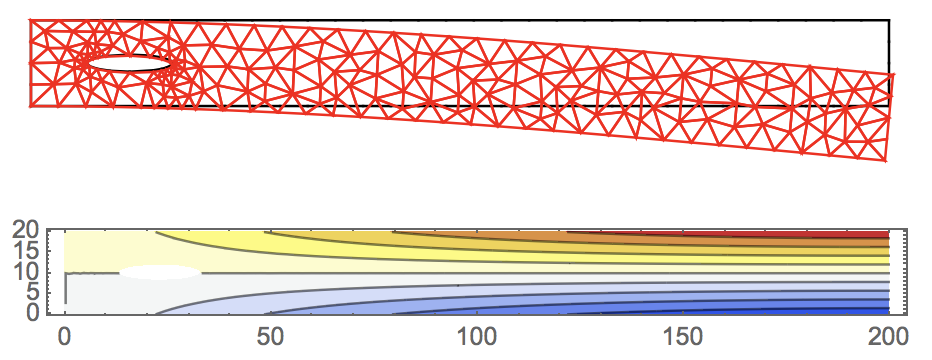
\includegraphics[width=0.5\textwidth]{beam_sample.png}
		\caption{Пример балки с повреждением: модель балки и диаграмма значений $\varepsilon_{11}$.}
		\label{fig:beam_sample}
	\end{figure}

	Разделим балку на 10 равных участков и обозначим $i$-ый участок $elem_i$:
	\begin{equation}
		elem_i = \{x: \ x \in [i \cdot 0.2\text{м}, (i+1) \cdot 0.2\text{м}]\}, \ i=0 \dots 9
	\end{equation}
	Аналогично разделим множество возможных значений $b$ на 3 равных участка:
	\begin{equation}
		ex_j = \{b: \ b \in [j \cdot 0.04\text{м} + 0.04\text{м}, (j+1) \cdot 0.04\text{м} + 0.04\text{м}]\}, \ j=0 \dots 2
	\end{equation}
	Задача ставится таким образом: по показаниям тензодатчиков требуется определить $i$ и $j$, такие что для координаты $x$ повреждения и его величины $ex$ верно, что $x \in elem_i$ и $ex \in ex_j$. Другими словами, надо указать, в каком участке балки и каком отрезке из множества возможных размеров повреждения лежит данное повреждение. Эта задача называется задачей классификации.
	
	\newpage
	\section{Принцип работы искусственных нейронных сетей}
	\label{sec:neural_networks}
	
	Искусственная нейронная сеть -- это математическая модель, построенная по принципу функционирования сетей нервных клеток живого организма. ИНС может быть представлена в виде взвешенного графа, вершины которого называются \textit{нейронами}, а веса ребер называются \textit{весами нейронов}. На Рис. \ref{fig:nn_architecture} представлена топология нейронных сетей, используемая в этой работе. Нейроны группируются в \textit{слои} (вертикальные столбцы на Рис. \ref{fig:nn_architecture}). Слои по расположению обозначаются соответственно как \textit{входной}, два \textit{скрытых} и \textit{выходной}, считая слева направо. В ходе работы нейронной сети сигнал поступает на входной слой и проходит последовательно через все слои, преобразуясь определенным образом. Такие нейронные сети называются сетями \textit{прямого распространения}.
	\begin{figure}[h]
		\begin{subfigure}{0.5\textwidth}
			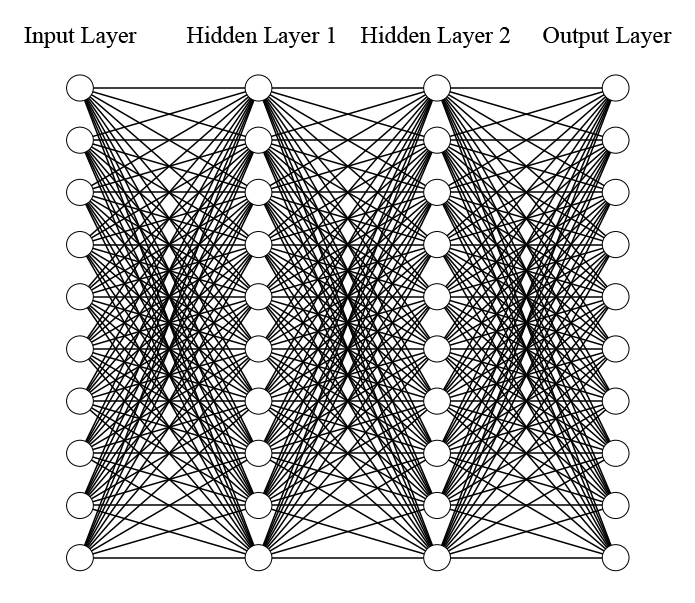
\includegraphics[width=\linewidth]{nn_architecture1.png}
			\caption{10 нейронов в выходном слое}
		\end{subfigure}
		\begin{subfigure}{0.5\textwidth}
			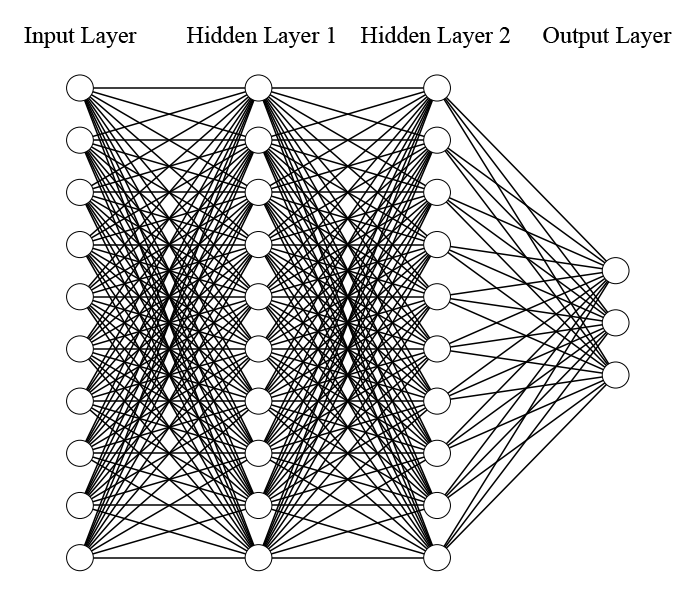
\includegraphics[width=\linewidth]{nn_architecture2.png}
			\caption{3 нейрона в выходном слое}
		\end{subfigure}
		\caption{Топология нейронных сетей, используемых в этой работе. Различие только в количестве нейронов в выходном слое (Output Layer).}
		\label{fig:nn_architecture}
	\end{figure}

	Нейронные сети -- это алгоритмы, работающие по принципу \textit{обучения с учителем}. Это значит, что перед тем как можно будет использовать алгоритм на практике, надо провести \textit{обучение}. Процесс обучения является итерационным процессом и состоит в корректировке весов нейронов. Для этого используется \textit{обучающая выборка} -- набор входных данных и соответствующий им набор заранее известных выходных данных. Этот набор также иногда называют набором пар «стимул-реакция».
	
	Для описания принципа работы ИНН необходимо дать описание нейрона, процесса \textit{прямого распространения сигнала} и \textit{обратного распространения ошибки}.
	
	\subsection{Устройство нейрона}

	Нейрон представляет собой линейную комбинацию поступающих в него сигналов $a_1^{l-1} \dots a_n^{l-1}$, взятых с коэффициентами $w_{1k}^l \dots w_{nk}^l$, называемых \textit{весами} нейрона. Здесь $w_{jk}^l$ обозначен вес, стоящий на ребре, соединяющем j-й нейрон слоя $(l-1)$ и k-й нейрон слоя $l$. К линейной комбинации иногда добавляют \textit{смещение} $b_k$, но в этой работе смещение не используется. От линейной комбинации затем берется \textit{функция активации} $f(x)$. Результат её вычисления и является выходным сигналом нейрона. Описанная схема работы приведена на Рис. \ref{fig:neuron_a}. Математический эквивалент этой схемы можно записать как (\ref{eq:neuron}).
	\begin{equation}\label{eq:neuron}
		a_k^l = f(\sum_{j=1}^{n} w_{jk}^l a_j^{l-1} + b_k)
	\end{equation}
	
	\begin{figure}[h]
		\begin{subfigure}[t]{0.6\textwidth}
			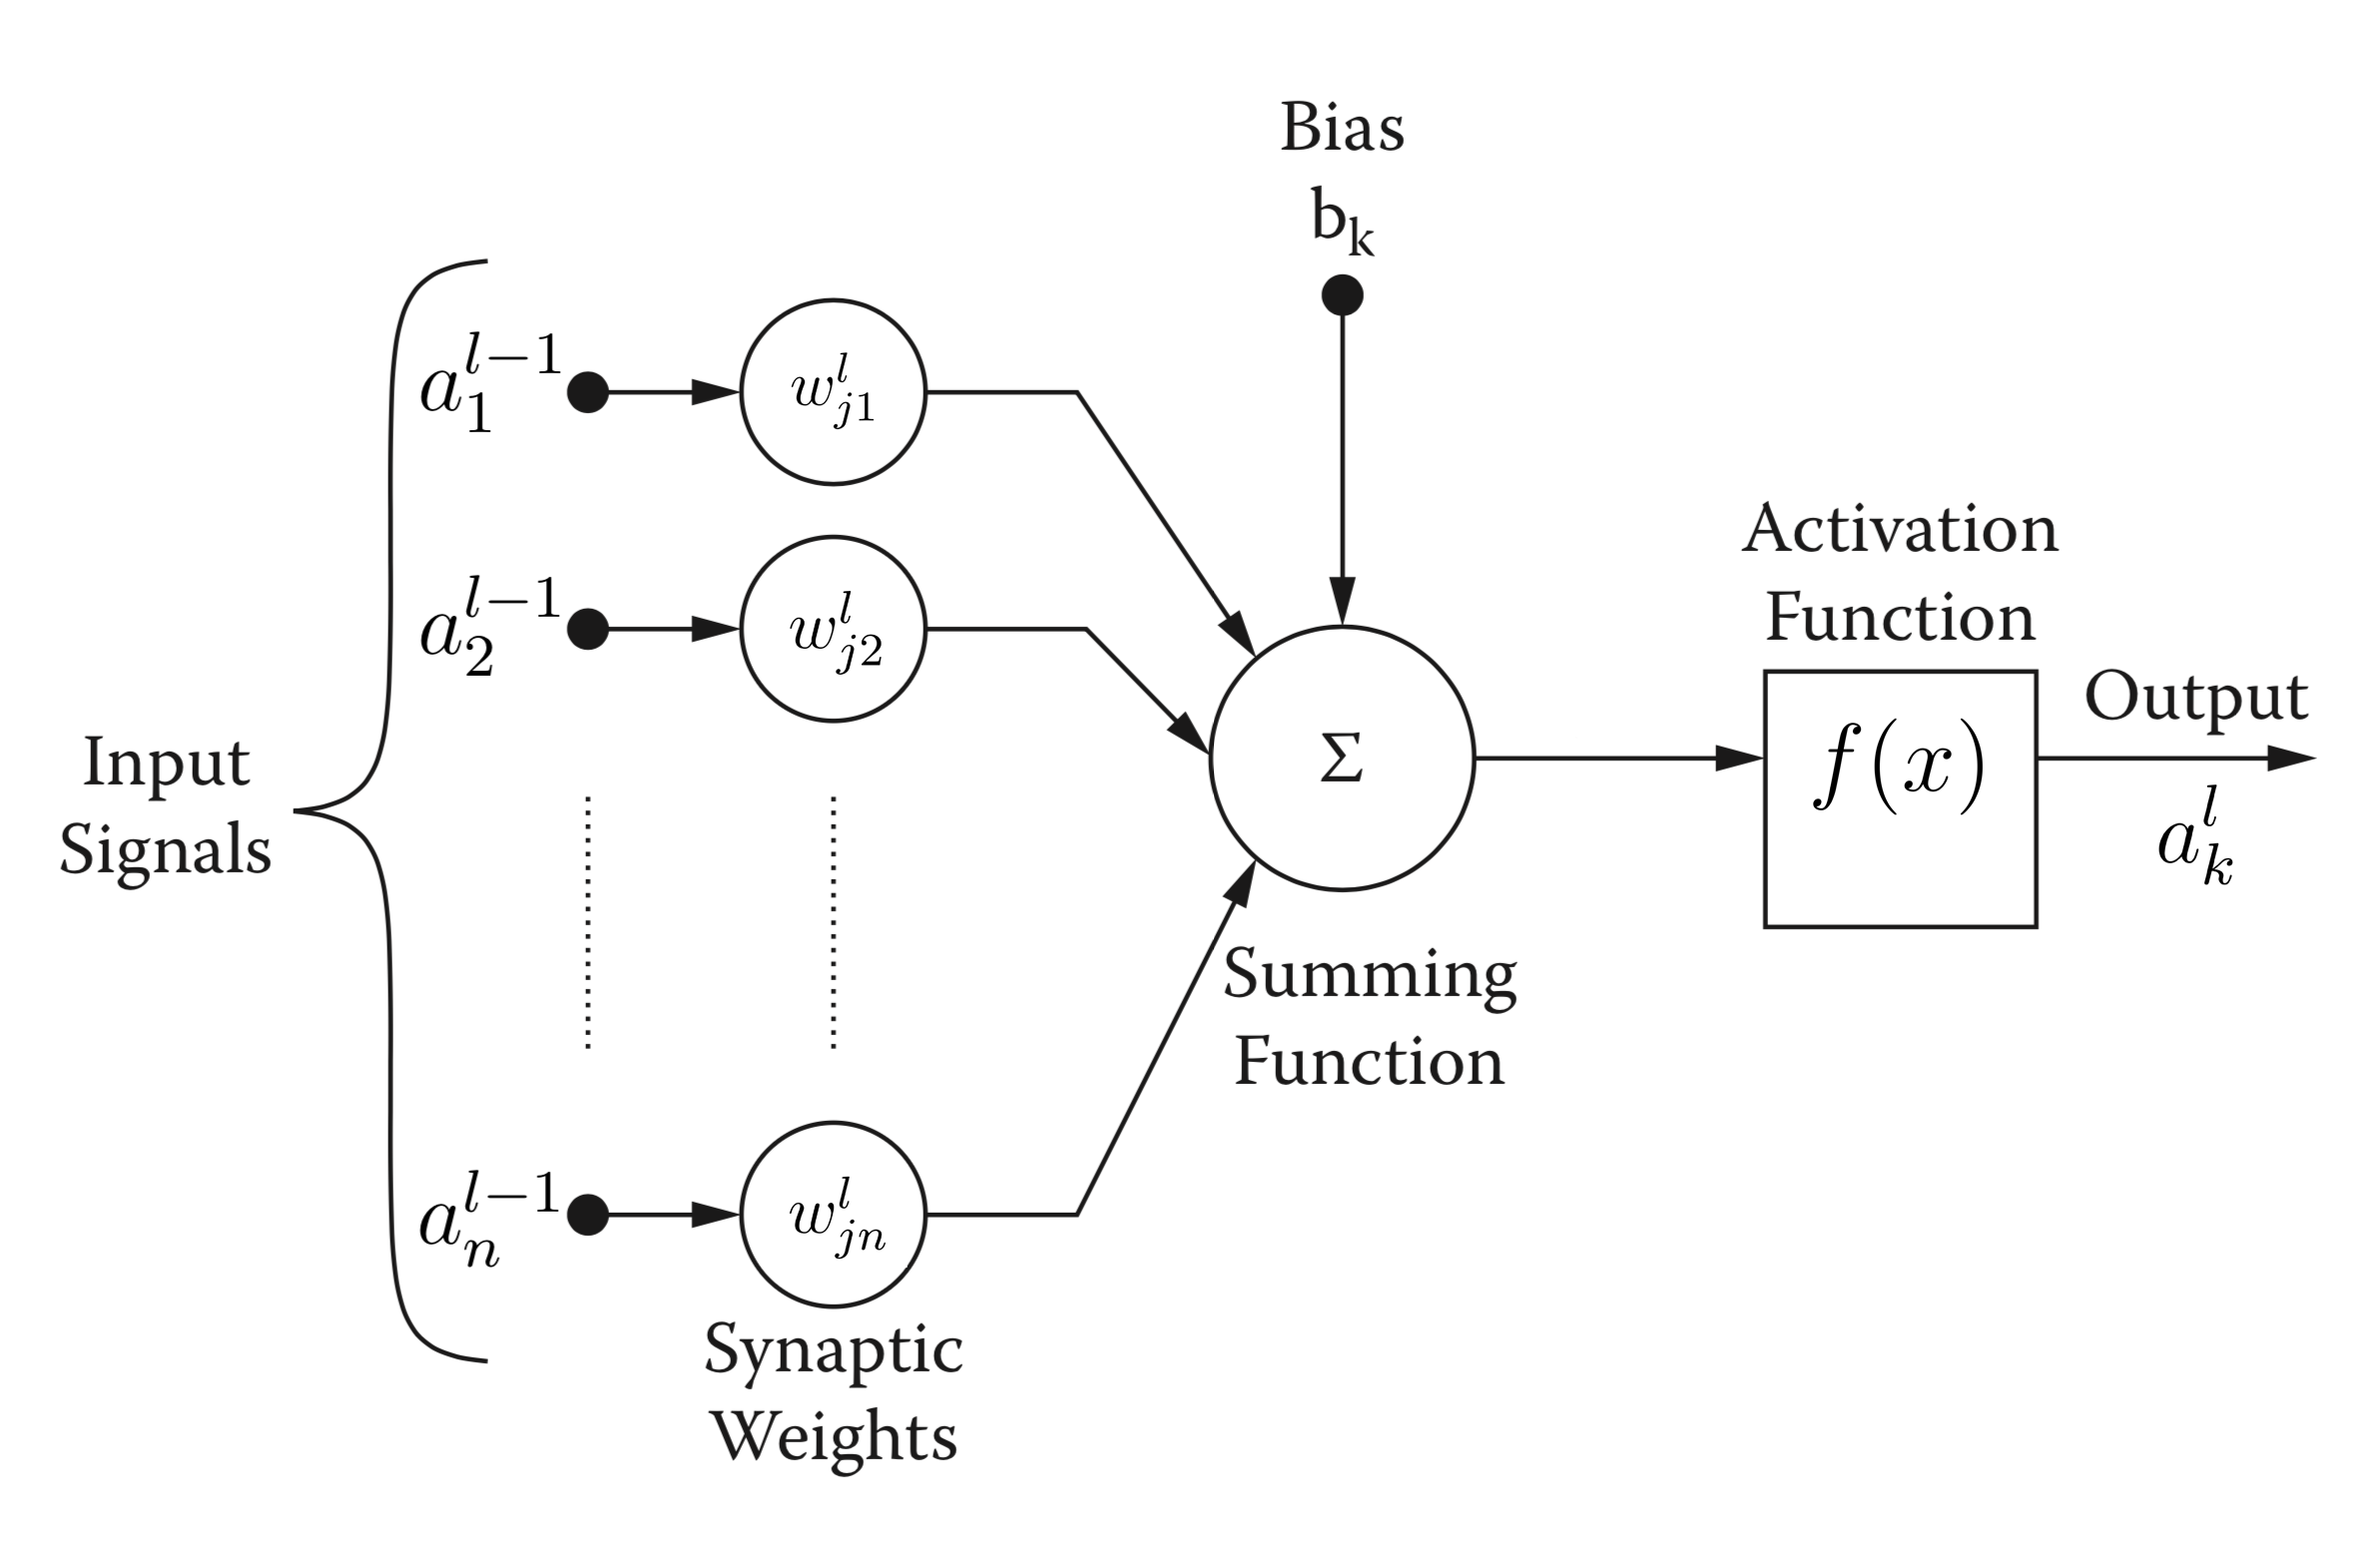
\includegraphics[width=\linewidth]{neuron.png}
			\caption{схема работы нейрона}
			\label{fig:neuron_a}
		\end{subfigure}
		\begin{subfigure}[t]{0.4\textwidth}
			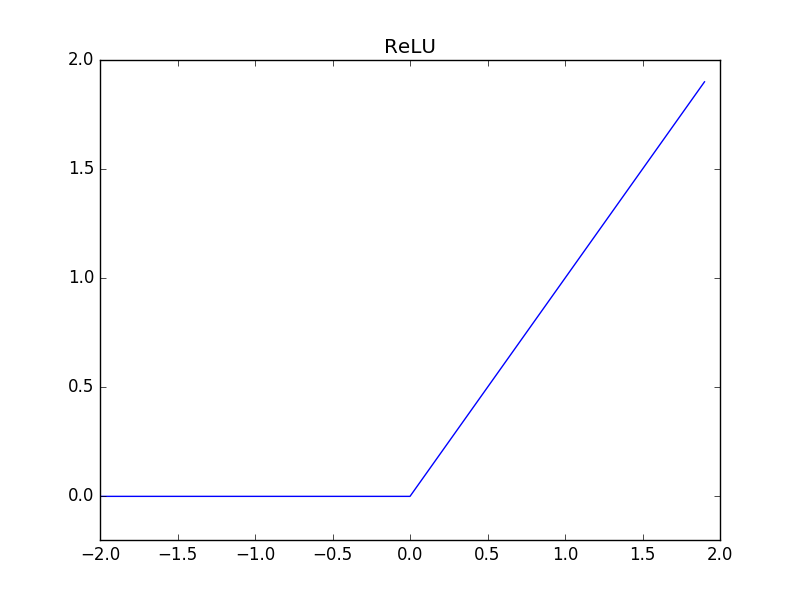
\includegraphics[width=\linewidth]{relu.png}
			\caption{график функции ReLU}
			\label{fig:neuron_b}
		\end{subfigure}
		\caption{Модель нейрона.}
		\label{fig:neuron}
	\end{figure}
	
	В представленной работе в качестве функции активации на скрытых слоях используется ReLU (Rectified Linear Unit):
	\begin{equation}
		a_k^l = relu(z_k^l) = max(0,z_k^l)
	\end{equation}
	Её график изображен на Рис. \ref{fig:neuron_b}. Эта функция была выбрана, поскольку она значительно ускоряет сходимость градиентного спуска во время обратного распространения ошибки по сравнению с функциями $sigmoid(x)$ и $tanh(x)$ \cite{imagenet_classification}.
	
	В качестве функции активации на выходном слое используется  softmax:
	\begin{equation}\label{eq:softmax}
		a_k^L = softmax(z_k^L) = \frac{e^{z_k^L}}{\sum_{c} e^{z_c^L}}
	\end{equation}
	Это функция, преобразующая вектор $z$ размерности $K$ в вектор $a$ той же размерности, где каждая координата $a_k$ полученного вектора представлена вещественным числом в отрезке $[0, 1]$ и сумма координат равна 1. Таким образом мы получаем на выходе распределение вероятностей. Здесь и далее буквой $L$ обозначается индекс последнего -- выходного -- слоя.
	
	\subsection{Прямое распространение сигнала}
	
	Прямое распространение сигнала -- это процесс преобразования входных данных в конечный результат работы нейросети. Прямое распространение используется как во время обучения -- чтобы найти вектор ошибки -- так и во время работы на новых данных, чтобы получить искомый результат.
	
	Посмотрим, как получается линейная комбинация в каждом из нейронов 1-го скрытого слоя:
	\begin{equation} \label{eq:first_sum}
		z_k^1 = \sum_j w_{jk}^1 a_j^0 \ ,
	\end{equation}
	где суммирование проводится по всем компонентам вектора входных данных $\vec{a^0}$. Линейные комбинации в каждом из нейронов 2-го скрытого слоя считаются точно так же, за исключением того, что вместо вектора входных данных берутся уже посчитанные линейные комбинации $z_j^1$, от которых взята функция активации $f^1$. В соответствии с (\ref{eq:neuron}) $a_j^1 = f^1(z_j^1)$:
	\begin{equation}
		\begin{gathered}
			z_k^2 = \sum_j w_{jk}^2 f^1(z_j^1) \\
			z_k^2 = \sum_j w_{jk}^2 a_j^1
		\end{gathered}
	\end{equation}
	Пусть теперь вместо одного вектора $\vec{a^0}$ на вход поступает набор вектор-столбцов, образующих матрицу $A_{ij}^0$. Будем называть этот набор входным \textit{пакетом данных}. Тогда (\ref{eq:first_sum}) можно переписать в форме матричного умножения:
	\begin{equation}
		\begin{gathered}
			Z^1 = W^1 A^0 \\
			Z_{kj}^1 = \sum_i W_{ki}^1 A_{ij}^0\ ,
		\end{gathered}
	\end{equation}
	То есть, чтобы получить линейную комбинацию в $k$-ом нейроне 1-го скрытого слоя, соответствующую $j$-ому вектор-столбцу из пакета входных данных $A^0$, необходимо $k$-ую строку матрицы $W^1$ умножить на $j$-ый вектор-столбец $A^0$. Строка $k$ матрицы $W^1$ состоит из весов на ребрах, соединяющих все нейроны входного слоя с $k$-ым нейроном 1-го скрытого слоя.
	
	При помощи матричных операций можно записать весь процесс прямого распространения сигнала:
	\begin{equation}
		\begin{gathered}
			Z^1 = W^1 A^0 \\
			A^1 = f^1(Z^1) \\
			Z^2 = W^2 A^1 \\
			A^2 = f^2(Z^2) \\
			Z^3 = W^3 A^2 \\
			A^3 = f^3(Z^3)
		\end{gathered}
	\end{equation}
	Или:
	\begin{equation}
		A^3 = f^3(W^3 f^2(W^2 f^1(W^1 A^0)))
	\end{equation}
	
	\subsection{Обратное распространение ошибки}
	
	Для корректировки весов нейронов в процессе обучения необходимо знать величину ошибки на выходном слое, то есть разницу между желаемым результатом и полученным. Напомним, что результат -- это некое дискретное распределение вероятностей, т. к. в качестве активационной функции на выходном слое используется softmax (\ref{eq:softmax}).
	
	В этой работе в качестве функции ошибки используется перекрестная энтропия (\ref{eq:entropy}). Поскольку она применяется к сигналу, полученному на выходном слое, можно подставить softmax из (\ref{eq:softmax}) и получить (\ref{eq:entropy_softmax}).
	\begin{equation}\label{eq:entropy}
		E(t_k, a_k^L) = - \sum_k t_k \ln a_k^L =
	\end{equation}
	\begin{equation}\label{eq:entropy_softmax}
		= - \sum_k t_k (z_k^L - \ln \sum_c e^{z_c^L})
	\end{equation}
	Здесь $t_k$ -- это желаемое распределение, которое имеет вид $\{0, \dots, 0, 1, 0, \dots, 0\}$, а $a_k^L$ -- полученное распределение, то есть сигнал на выходе последнего слоя $L$. Перекрестная энтропия здесь используется в качестве меры несовпадения между распределениями $t_k$ и $a_k^L$.
	
	Для корректировки весов нейронов в процессе обучения к каждому весу прибавляется поправка вида
	\begin{equation}\label{eq:gradient_descent}
		\Delta w_{jk}^l = - \eta \frac{\partial E}{\partial a_k^l}
	\end{equation}
	Поправки рассчитываются заново для каждого нового пакета входных данных. Процесс, описываемый формулой (\ref{eq:gradient_descent}), называется методом \textit{градиентного спуска}, а константа $\eta$ -- \textit{шагом} градиентного спуска. Рассмотрим как вычисляется производная из (\ref{eq:gradient_descent}) для последнего слоя и для скрытых слоев.
	
	На последнем (выходном) слое
	\begin{equation}
		\frac{\partial E}{\partial w_{jk}^L} = \frac{\partial E}{\partial z_k^L} \frac{\partial z_k^L}{\partial w_{jk}^L}
	\end{equation}
	Посчитаем первый множитель, продифференцировав (\ref{eq:entropy}):
	\begin{equation}
		\begin{gathered}
			\frac{\partial E}{\partial z_k^L} = - \sum_d t_d (I_{d = k} - \frac{1}{\sum_c e^{z_c^L}} e^{z_k^L}) = \\
			= - \sum_d t_d (I_{d = k} - a_k^L) = \\
			= \sum_d t_d a_k^L - \sum_d t_d I_{d = k} = \\
			= a_k^L \sum_d t_d - t_k = \\
			= a_k^L - t_k
		\end{gathered}
	\end{equation}
	Здесь $I_{d = k}$ -- единичный тензор. Второй множитель считается тривиально:
	\begin{equation}
		\frac{\partial z_k^L}{\partial w_{jk}^L} = a_j^{L-1}
	\end{equation}
	Тогда, обозначив
	\begin{equation}
		\delta_k^L = \frac{\partial E}{\partial z_k^L} = a_k^L - t_k,
	\end{equation}
	можем записать результат в виде:
	\begin{equation}\label{eq:derivative_output}
		\frac{\partial E}{\partial w_{jk}^L} = \delta_k^L a_j^{L-1}
	\end{equation}
	
	Проделаем аналогичные вычисления для скрытого слоя $l - 1$.
	\begin{equation}
		\frac{\partial E}{\partial w_{ij}^{l-1}} = \frac{\partial E}{\partial a_j^{l-1}} \frac{\partial a_j^{l-1}}{\partial z_j^{l-1}} \frac{\partial z_j^{l-1}}{\partial w_{ij}^{l-1}}
	\end{equation}
	\begin{equation}
		\begin{gathered}
			\frac{\partial E}{\partial a_j^{l-1}} = \sum_k \frac{\partial E}{\partial z_k^l} \frac{\partial z_k^l}{\partial a_j^{l-1}} \\
			= \sum_k \delta_k^l w_{jk}^l
		\end{gathered}
	\end{equation}
	\begin{equation}
		\frac{\partial a_j^{l-1}}{\partial z_j^{l-1}} = f'(z_j^{l-1})
	\end{equation}
	\begin{equation}
		\frac{\partial z_j^{l-1}}{\partial w_{ij}^{l-1}} = a_i^{l-2}
	\end{equation}
	Объединяя всё вместе, получаем:
	\begin{equation}\label{eq:together}
		\frac{\partial E}{\partial w_{ij}^{l-1}} = a_i^{l-2} f'(z_j^{l-1}) \sum_k \delta_k^l w_{jk}^l
	\end{equation}
	Обозначим
	\begin{equation}
		\delta_j^{l-1} = \frac{\partial E}{\partial a_j^{l-1}} \frac{\partial a_j^{l-1}}{\partial z_j^{l-1}} = f'(z_j^{l-1}) \sum_k \delta_k^l w_{jk}^l
	\end{equation}
	и перепишем выражение (\ref{eq:together}):
	\begin{equation}\label{eq:derivative_hidden}
		\frac{\partial E}{\partial w_{ij}^{l-1}} = \delta_j^{l-1} a_i^{l-2}
	\end{equation}
	
	Таким образом, мы научились вычислять поправки (\ref{eq:gradient_descent}) для нейронов выходного и скрытых слоев, используя производные, посчитанные в (\ref{eq:derivative_output}) и (\ref{eq:derivative_hidden}) соответственно. Заметим что, как оказалось, для расчета (\ref{eq:derivative_output}) требуется знать только желаемое и полученное распределения. А вот для расчета (\ref{eq:derivative_hidden}) необходимо посчитать $\delta_j^{l-1}$, которая выражается через $\delta_1^l \dots \delta_N^l$ следующего слоя, где $N$ -- количество нейронов в следующем слое. И так для каждого слоя: чтобы посчитать производные по формулам (\ref{eq:derivative_output}) и (\ref{eq:derivative_hidden}), по сути надо сначала посчитать производные для следующего слоя. Поэтому расчет поправок производится справа налево: сначала для выходного слоя, потом для последнего скрытого и т. д. Отсюда становится ясно происхождение названия: метод обратного распространения ошибки (backpropagation method).
	
	\newpage
	\section{Порядок действий для решения поставленной задачи}
	\label{sec:solving_problem}
	
	\subsection{Получение обучающих выборок}
	Выборка -- это набор пар вида \{параметры повреждения, показания тензодатчиков\}. В каждой такой паре параметры дефекта выбираются случайно. Для каждой пары строится конечно-элементная модель балки в Wolfram Mathematica и снимаются показания тензодатчиков, как описано в разделе \ref{sec:formulation_problem}.
	
	В первой выборке $set_0$ варьируются координаты $(x, y)$ центра повреждения (Рис. \ref{fig:beam_sample}), а остальные параметры повреждения постоянны. В базу данных для каждой пары из выборки сохраняется одна строка, состоящая из координат повреждения и показаний тензодатчиков (Рис. \ref{bd_sample}). Показания 0-го датчика не используются при обучении, потому что по постановке задачи они всегда нулевые. Координата $y$ также игнорируется, а $x$ преобразуется в индекс $i$ участка $elem_i$ целочисленным делением на 20. Индекс $i$ называется меткой (label) и используется в качестве правильного ответа при обучении. Были сформированы два варианта этой выборки для случая $F = 2\text{кг}$ и $F = 4\text{кг}$, то есть для разных граничных условий на правом конце балки (см. раздел \ref{sec:formulation_problem}). Это позволило определить, при каких граничных условиях предсказания получаются более точными. Эти выборки используются для задачи предсказания местонахождения повреждения при фиксированной величине.
	\begin{figure}[h]
		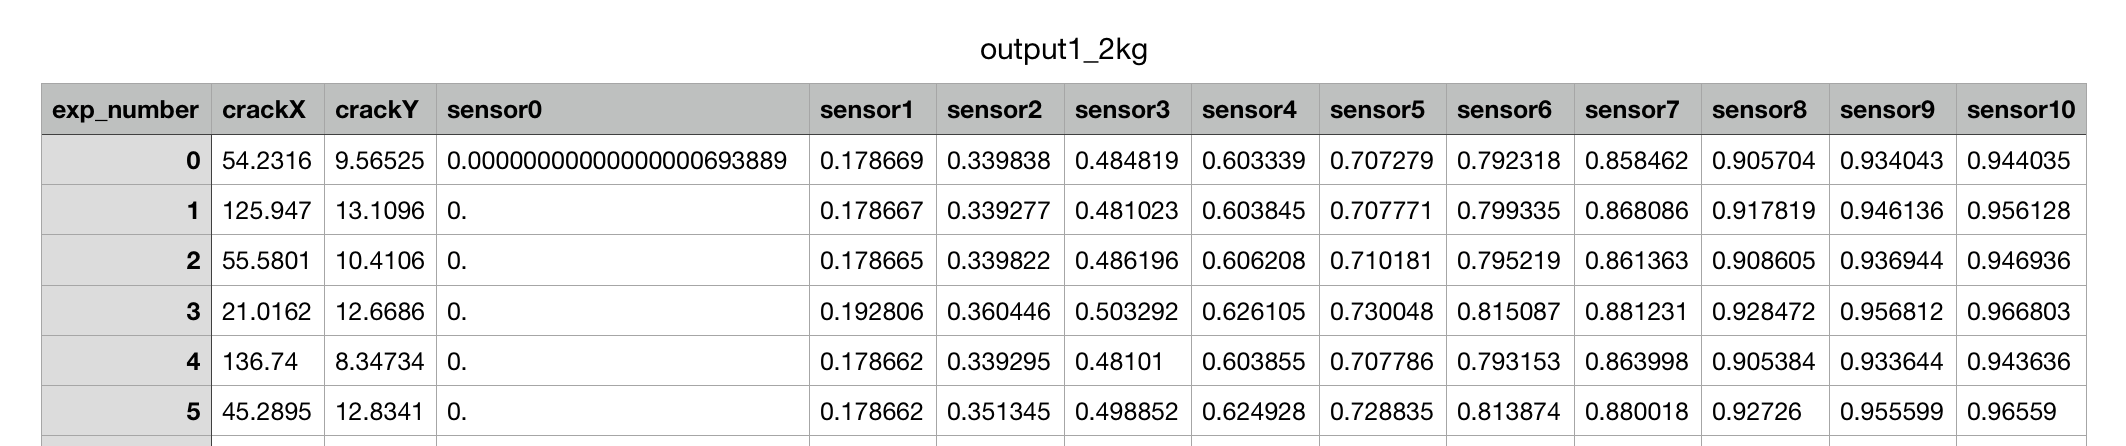
\includegraphics[width=\textwidth]{db_sample.png}
		\caption{Пример содержания базы данных.}
		\label{bd_sample}
	\end{figure}

	Была также сформирована выборка $set_1$, отличающаяся от $set_0$ тем, что дополнительно варьировался размер повреждения. 	Соответственно, в базу данных добавился столбец crack\_extent. Эта выборка используется для задачи предсказания местонахождения повреждения при неизвестном размере повреждения.
 
 	Наконец, были сформированы выборки $set_{2i}, i = 0 \dots 9$. Они аналогичны $set_1$, за исключением того, что координаты $x$ дефектов выбирались таким образом, что $x \in elem_i$. При обучении по этой выборке значения столбца преобразовывались в метку $j$ размера дефекта (см. раздел \ref{sec:formulation_problem}). Эти выборки используются для задачи предсказания размера дефекта при известном местонахождении (см. раздел \ref{sec:results_location_extent}).
 	
 	\subsection{Выставление параметров нейронных сетей}
 	Параметрами нейронных сетей является количество скрытых слоев (слоев между входным и выходным слоями), количество нейронов в каждом слое, функции активации, метод корректировки весов, размер пакета входных данных. Параметры подбираются эмпирически для каждой задачи. В этой работе во всех нейронных сетях использовалась архитектура с двумя скрытыми слоями, по 10 нейронов в каждом, с функциями активации ReLU на скрытых слоях и softmax на выходном слое (см. раздел \ref{sec:neural_networks}). Размер пакета входных данных был выбран 64 для нейронных сетей, обученных на выборках $set_0$ и $set_1$ и 32 для нейронных сетей, обученных на выборках $set_{20} \dots set_{29}$.
 	
 	В качестве метода корректировки весов вместо обычного метода градиентного спуска (см. раздел \ref{sec:neural_networks}) использовался метод адаптивного градиентного спуска (АГС) \cite{adagrad}. Улучшение состоит в том, что шаг $\eta$ зависит от конкретного параметра (входа нейрона в данном случае) и временного шага. То есть, если обычный градиентный спуск работает по принципу
 	\begin{equation}
 		\Delta w_{jk}^l = - \eta \frac{\partial E}{\partial a_l^l}\ ,
 	\end{equation}
 	то АГС модифицирует шаг градиентного спуска на каждом временном шаге для каждого $w_{jk}^l$ по принципу:
 	\begin{equation}\label{eq:adagrad}
 		\Delta w_{jk}^l = - \frac{\eta}{\sqrt{G_{t,ii} + \varepsilon}} \frac{\partial E}{\partial a_l^l}\ ,
 	\end{equation}
 	где $G_{t,ii}$ -- диагональная матрица, где каждый диагональный элемент $g_{ii}$ является суммой квадратов градиентов, вычисленных для $w_{jk}^l$ за все моменты времени до момента $t$. Здесь $\varepsilon$ это малое слагаемое, введенное для избежания деления на 0. Таким образом, АГС подстраивает шаг таким образом, чтобы со временем замедлять слишком быстро меняющиеся веса. АГС показал наилучшие результаты на полученных выборках данных.
 	
 	\subsection{Отслеживание процесса обучения}
	Процесс обучения нейронных сетей является итерационным процессом. На каждой итерации через нейронную сеть пропускается вся обучающая выборка. Обучающая выборка подается порциями, равными размеру входного пакета данных. В ходе обучения происходит корректировка весов нейронов.
	
	В ходе обучения после каждой итерации проверяется работа нейросети на \textit{тестовой выборке}, которая не участвует в процессе обучения. Это делается для того, чтобы отслеживать прогресс обучения на всегда ``новых'' для нейросети данных. В этой работе каждая выборка из 10 000 пар делилась на обучающую и тестовую в отношении 4 : 1, то есть на каждой итерации 8000 пар использовались для обучения и 2000 для проверки.
	
	В ходе обучения и для обучающей, и для тестовой выборки отслеживается по два параметра. Первый параметр называется \textit{потери} (loss), и он равен среднему по всей выборке значению функции ошибки (\ref{eq:entropy_softmax}). Второй параметр называется \textit{точность} (accuracy), и он равен среднему по выборке проценту правильных ответов. Ответом нейросети считается индекс, имеющий в распределении наибольшую вероятность (см. раздел \ref{sec:formulation_problem}).
	
	Процесс обучения нейросетей продолжается до тех пор, пока не начнется \textit{переобучение}, либо пока не перестанет расти точность. Переобучение -- это явление, при котором нейронная сеть излишне приспосабливается к обучающим данным и потери на тестовой выборке начинают расти, а точность падать, хотя на обучающей выборке при этом может наблюдаться дальнейшее уменьшение потерь и рост точности. При переобучении пропадает способность нейронных сетей к обобщению. Особенностью метода АГС (\ref{eq:adagrad}) является то, что часто шаг градиентного спуска в какой-то момент становится настолько мал, что обучение фактически прекращается. Это и произошло при применении его в этой работе (см. раздел \ref{sec:results}).
	
	\newpage
	\section{Результаты}
	\label{sec:results}
	
	После того как нейросети обучены, можно использовать их по назначению. То есть, запускать прямое распространение сигнала (см. раздел \ref{sec:neural_networks}) без последующей корректировки весов нейронов. Результаты их использования, а также графики потерь и точности, полученные при обучении, приведены в этом разделе.
	
	\subsection{Прогнозирование местонахождения повреждения при его фиксированной величине}
	\label{sec:results_location}
	
	Обучение было проведено для двух вариантов нагрузки: 2кг и 4кг (Рис. \ref{fig:nn1_training_metrics}).	На верхних графиках представлена зависимость потерь от номера итерации, на нижних -- точности от номера итерации. Всего было проведено 10 000 итераций. Видно, что линии, соответствующие тестовой выборке, немного отстают от обучающей, но при этом разрыв значительно не увеличивается. Это говорит о том, что \textit{переобучения} не происходит. То есть, не происходит излишнего приспособления нейросети к обучающим данным, из-за которого она перестает делать правильные предсказания на тестовых.
	\begin{figure}[h]
		\begin{subfigure}{0.5\textwidth}
			\includegraphics[width=\linewidth]{{nn1_2kg_adagrad0.1_batch64_10000}.png}
			\caption{нагрузка 2кг}
		\end{subfigure}
		\begin{subfigure}{0.5\textwidth}
			\includegraphics[width=\linewidth]{{nn1_4kg_adagrad0.1_batch64_10000}.png}
			\caption{нагрузка 4кг}
		\end{subfigure}
		\caption{Графики потерь и точности на обучающей и тестовой выборке для нейронных сетей, обученных на балках с разной нагрузкой.}
		\label{fig:nn1_training_metrics}
	\end{figure}

	Удалось добиться следующих результатов на 10 000-й итерации: \\
	
	\begin{tabular}{| l | l | l | l |}
		\hline
		Нагрузка & Выборка & Потери & Точность \\
		\hline
		2кг & Train & 0.678 & 73.550\% \\
		\hline
		2кг & Test & 0.729 & 70.376\% \\
		\hline
		4кг & Train & 0.715 & 70.450\% \\
		\hline
		4кг & Test & 0.733 & 69.200\% \\
		\hline
	\end{tabular} \\

	Видно, что при обучении с нагрузкой 2кг удалось получить небольшой выигрыш в точности по сравнению с нагрузкой 4кг. Выигрыш составил 1.176\%. Далее будет рассматриваться только нагрузка 2кг.
	
	Таким образом, при выборе одного поврежденного участка из 10, нейросеть дает верный результат примерно в 70\% случаев.
	
	Интересно посмотреть, какие предсказания сделает нейросеть на вручную выбранных данных, а не сгенерированных случайно. На Рис. \ref{fig:nn1_damage_30_10} приведен такой пример. Вектор входных данных состоит из показаний датчиков; вектор предсказаний содержит выходные значения сигналов на последнем слое нейросети (Рис. \ref{fig:nn1_damage_30_10_a}). Вектор предсказаний затем  преобразуется в распределение вероятностей функцией softmax (\ref{eq:softmax}) и отображается на диаграмме. По диаграмме видно, что наиболее вероятно центр повреждения лежит в участке под индексом 1 -- это соответствует истине.
	\begin{figure}[h]
		\begin{subfigure}[t]{0.6\textwidth}
			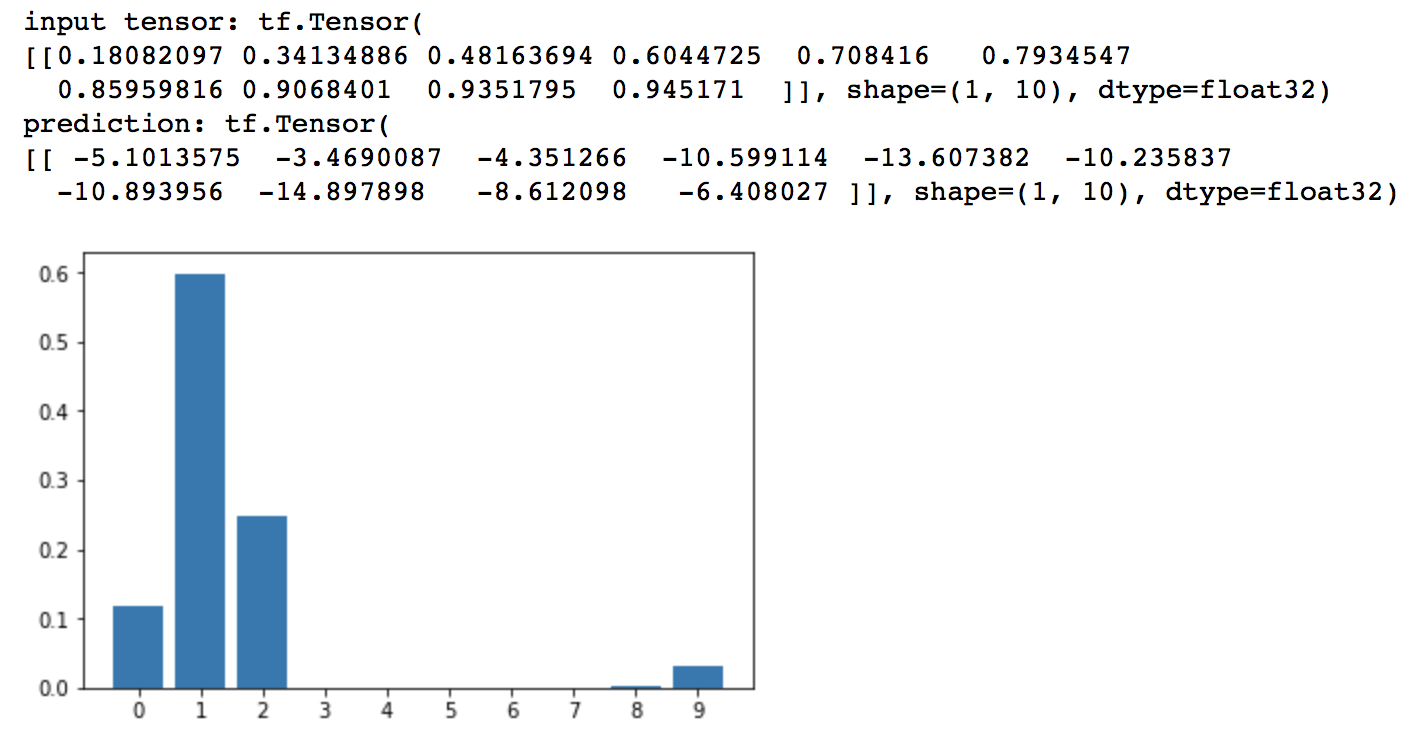
\includegraphics[width=\linewidth]{nn1_damage_30_10.png}
			\caption{предсказание}
			\label{fig:nn1_damage_30_10_a}
		\end{subfigure}
		\begin{subfigure}[t]{0.4\textwidth}
			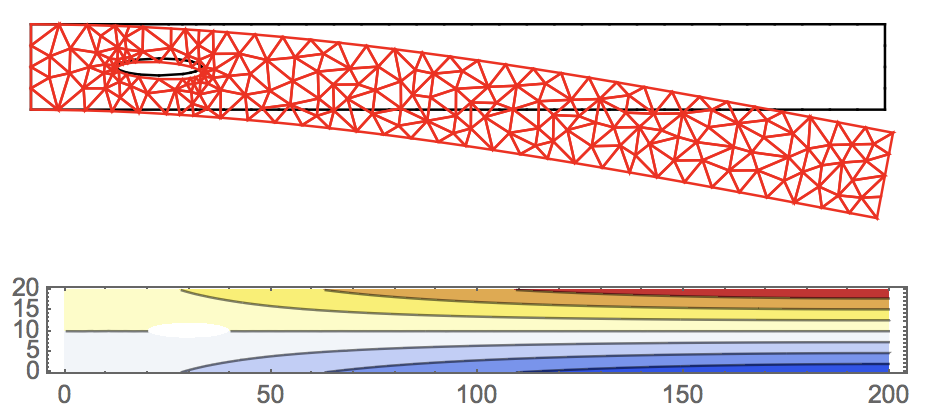
\includegraphics[width=\linewidth]{ds1_damage_30_10.png}
			\caption{соответствующая балка}
		\end{subfigure}
		\caption{Тест на балке с повреждением в координатах $(30, 10)$.}
		\label{fig:nn1_damage_30_10}
	\end{figure}

	В этом случае предсказание весьма уверенное -- лидирующая вероятность более чем на 0.3 превышает следующую за ней. Рассмотрим случай менее уверенного предсказания -- для повреждения в координатах $(150, 10)$ (Рис. \ref{fig:nn1_damage_150_10}). Выбором разных $y$-координат повреждения (Рис. \ref{fig:nn1_damage_150_6}, \ref{fig:nn1_damage_150_14}) убеждаемся, что точность предсказаний увеличивается при удалении повреждения от срединной линии балки. Об этом говорит значение вероятности нахождения повреждения в участке под индексом 7, обозначенной как $P(elem_7)$.
	\begin{figure}[h]
		\begin{subfigure}{0.33\textwidth}
			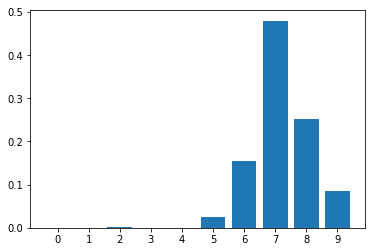
\includegraphics[width=\linewidth]{nn1_damage_150_6.png}
			\caption{$y=6: P(elem_7)\approx0.5$}
			\label{fig:nn1_damage_150_6}
		\end{subfigure}
		\begin{subfigure}{0.33\textwidth}
			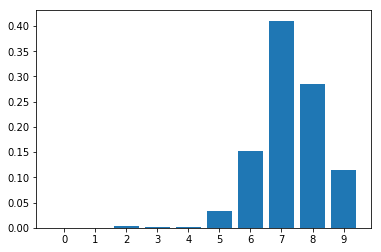
\includegraphics[width=\linewidth]{nn1_damage_150_10.png}
			\caption{$y=10: P(elem_7)\approx0.4$}
			\label{fig:nn1_damage_150_10}
		\end{subfigure}
		\begin{subfigure}{0.33\textwidth}
			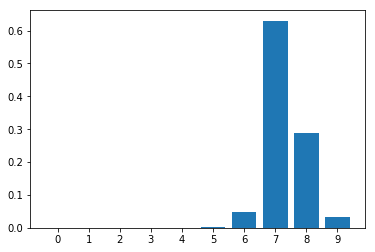
\includegraphics[width=\linewidth]{nn1_damage_150_14.png}
			\caption{$y=14: P(elem_7)\approx0.6$}
			\label{fig:nn1_damage_150_14}
		\end{subfigure}
		\caption{Тест на балках с повреждениями в $x=150$ и разных $y$.}
		\label{fig:nn1_damage_150}
	\end{figure}

	\begin{wrapfigure}{r}{0.33\textwidth} 
		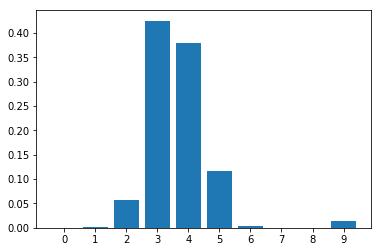
\includegraphics[width=\linewidth]{nn1_damage_80_10.png}
		\caption{Тест на балке с повреждением в координатах $(80, 10)$.}
		\label{fig:nn1_damage_80_10}
	\end{wrapfigure}
	Интересно также рассмотреть случай, когда центр повреждения лежит не посередине какого-либо участка, а ровно на границе между двумя. Например, возьмем центр в $x=80$, то есть на границе между 3 и 4 участками (Рис. \ref{fig:nn1_damage_80_10}). По распределению вероятностей видно, что столбцы, отвечающие 3 и 4 участкам, имеют примерно равные высоты, отличающиеся не более чем на 0.05. Это наблюдение можно использовать на практике: при близких соседних вероятностях, когда прочие вероятности малы, скорее всего повреждение находится где-то посередине.
	
	Наконец, посмотрим на предсказание нейросети для балки, вообще не имеющей повреждения (Рис. \ref{fig:nn1_no_damage}). Это предсказание весьма логично. Ведь, напомним, нейросеть априори ``полагает'', что в балке есть повреждение. Стало быть, не находя признаков этого повреждения, она смещает свой прогноз в ту часть балки, где повреждение наименее всего влияет на показания датчиков, то есть в правый конец.
	\begin{figure}[h]
		\begin{subfigure}[t]{0.6\textwidth}
			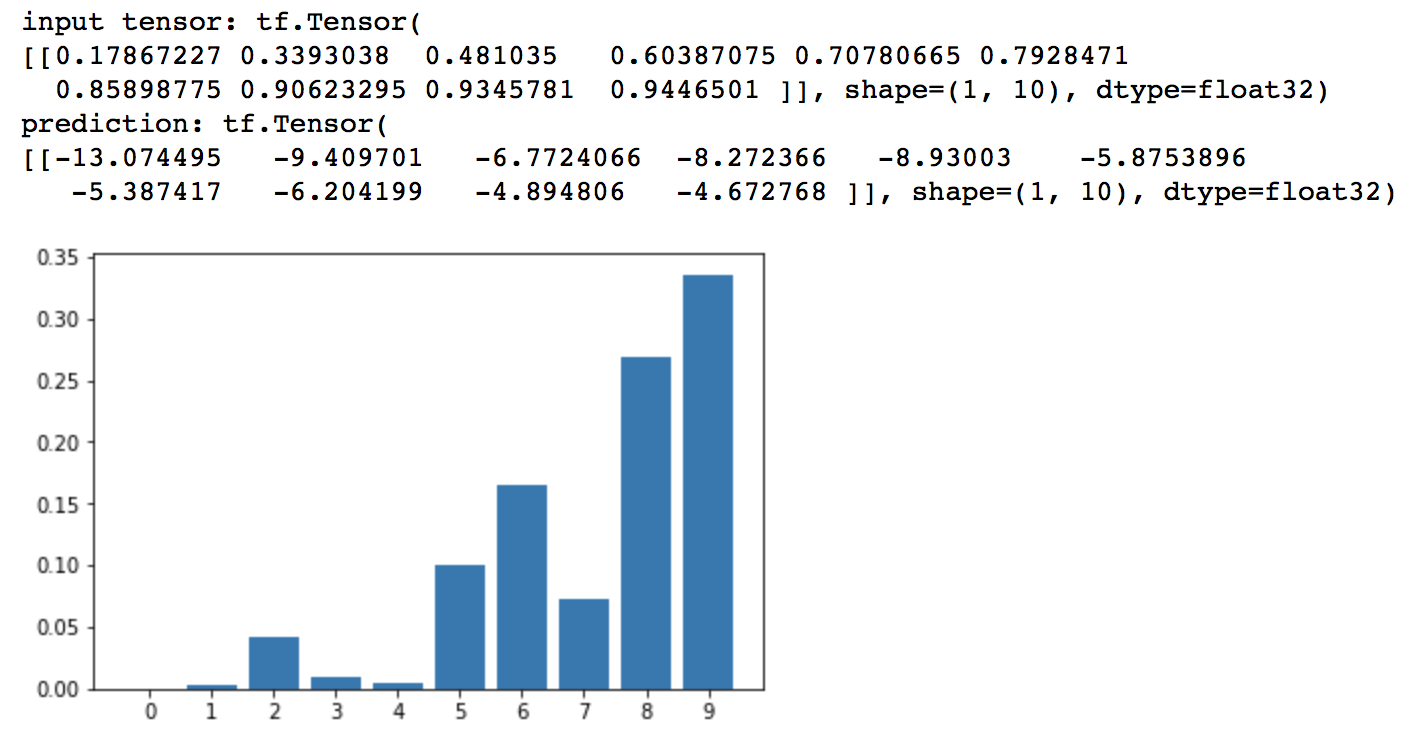
\includegraphics[width=\linewidth]{nn1_no_damage.png}
			\caption{предсказание}
			\label{fig:nn1_no_damage_a}
		\end{subfigure}
		\begin{subfigure}[t]{0.4\textwidth}
			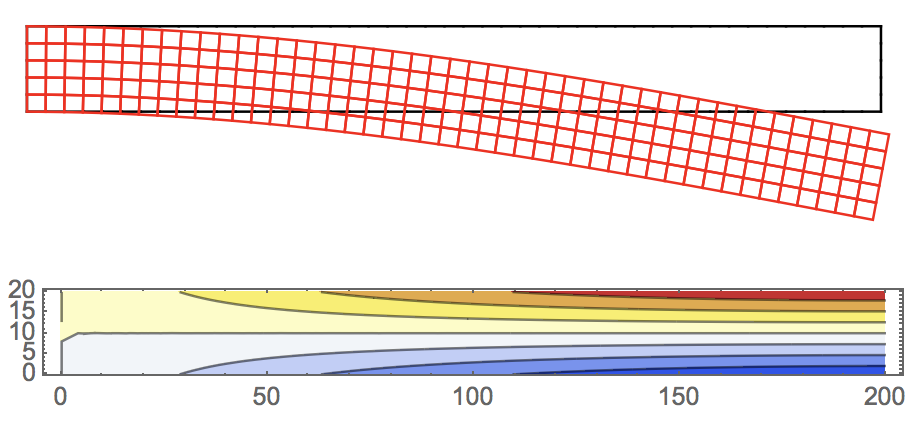
\includegraphics[width=\linewidth]{ds1_no_damage.png}
			\caption{соответствующая балка}
		\end{subfigure}
		\caption{Тест на балке без повреждения.}
		\label{fig:nn1_no_damage}
	\end{figure}

	Несмотря на логичность, нейросеть, очевидно, плохой инструмент для проверки факта наличия дефекта. Вместо этого надо просто перед применением нейросети проверять, не совпадает ли вектор входных данных с вектором из первой строчки Рис. \ref{fig:nn1_no_damage_a} в пределах погрешности датчиков. Если совпадает, значит применение нейросети вовсе не требуется -- повреждение отсутствует.
	
	\subsection{Прогнозирование местонахождения и величины повреждения}
	\label{sec:results_location_extent}
	
	Для решения усложненной задачи поиска двух параметров повреждения использовалась следующая система.
	
	\begin{wrapfigure}{l}{0.5\textwidth} 
		\includegraphics[width=\linewidth]{{nn2_2kg_adagrad0.1_batch64_10000}.png}
		\caption{Графики потерь и точности на обучающей и тестовой выборке для $nn_1$.}
		\label{fig:nn2_training_metrics}
	\end{wrapfigure}
	
	Сначала нейросеть находит участок с повреждением, аналогично тому как это делалось в разделе \ref{sec:results_location}. При этом помимо координат $(x, y)$ добавился третий, также случайно варьируемый параметр $ex$, отвечающий за величину повреждения (см. раздел \ref{sec:formulation_problem}). Обозначим эту выборку $set_1$, а соответствующую нейросеть -- $nn_1$.
	
	Также для каждого участка $i$ была обучена отдельная нейросеть $nn_{2i}$ по выборке $set_{2i}$, в которой $(x, y)\in elem_i,\ ex\in D_{ex}\ (D_{ex}\text{ -- вся область определения }ex)$. На выходе эти нейросети дают только оценку величины повреждения.
	
	Таким образом, если мы обозначим вектор входных данных как $a_k^0$, процесс получения результата можно описать двумя шагами: \\
	
	\begin{enumerate}[itemsep=0cm, topsep=0.2cm]
		\item Подаем тензор $a_k^0$ на вход нейросети $nn_1 \Rightarrow$ получаем индекс $i$ участка, содержащего центр повреждения.
		\item Подаем тензор $a_k^0$ на вход нейросети $nn_{2i} \Rightarrow$ получаем оценку величины повреждения $ex$.
	\end{enumerate}

	На графиках (Рис. \ref{fig:nn2_training_metrics}) показан процесс обучения нейросети $nn_1$. Результаты, полученные на 10 000-й итерации, показаны в таблице: \\
	
	\begin{tabular}{| l | l | l | l |}
		\hline
		Нагрузка & Выборка & Потери & Точность \\
		\hline
		2кг & Train & 0.901 & 62.513\% \\
		\hline
		2кг & Test & 0.955 & 61.150\% \\
		\hline
	\end{tabular} \\

	За счет дополнительного случайного параметра $ex$ точность упала примерно на 9\% по сравнению с аналогичными результатами в разделе \ref{sec:results_location}.
	
	\begin{figure}[h]
		\begin{subfigure}{0.33\textwidth}
			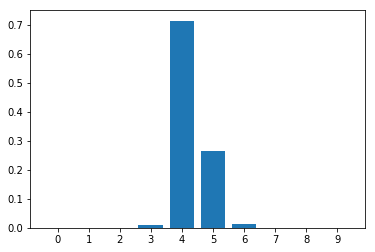
\includegraphics[width=\linewidth]{nn2_damage_90_14_6.png}
			\caption{$ex=6: P(elem_4)\approx0.7$}
		\end{subfigure}
		\begin{subfigure}{0.33\textwidth}
			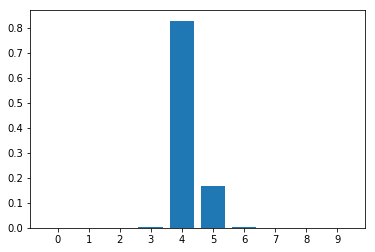
\includegraphics[width=\linewidth]{nn2_damage_90_14_10.png}
			\caption{$ex=10: P(elem_4)\approx0.8$}
		\end{subfigure}
		\begin{subfigure}{0.33\textwidth}
			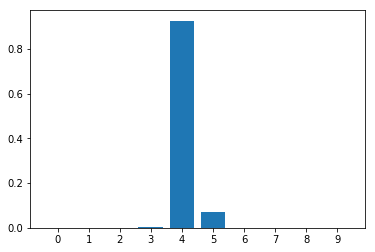
\includegraphics[width=\linewidth]{nn2_damage_90_14_14.png}
			\caption{$ex=14: P(elem_4)\approx0.85$}
		\end{subfigure}
		\caption{Тест нейросети $nn_1$ на балках с повреждениями в $x=90,\ y=14$ и разными $ex$.}
		\label{fig:nn2_damage_90_14}
	\end{figure}

	\begin{wrapfigure}{r}{0.5\textwidth} 
		\includegraphics[width=\linewidth]{{nn3_2kg_elem4_adagrad0.1_batch64_10000}.png}
		\caption{Графики потерь и точности на обучающей и тестовой выборке для $nn_{24}$.}
		\label{fig:nn3_training_metrics}
	\end{wrapfigure}
	Будем обозначать повреждения тройками $\{x, y, ex\}$. Проверим, например, правильность предсказаний для трех моделей с параметрами повреждений $\{90, 14, 6\}$, $\{90, 14, 10\}$, $\{90, 14, 14\}$. Нейросеть для всех трех моделей дала правильный результат (Рис. \ref{fig:nn2_damage_90_14}). Что характерно, точность предсказаний увеличивается при увеличении размера повреждения.

	Поскольку результат -- участок балки под индексом 4, для предсказания величины повреждения выбираем нейросеть $nn_{24}$. Графики обучения приведены на Рис. \ref{fig:nn3_training_metrics}. Архитектура этой нейросети отличается от предыдущих только числом нейронов в выходном слое -- 3 вместо 10 -- и размером батча -- 32 вместо 64. По Рис. \ref{fig:nn3_damage_90_14} видно, что нейросеть дала верные результаты на трех выбранных моделях.

	\begin{figure}[h]
		\begin{subfigure}{0.33\textwidth}
			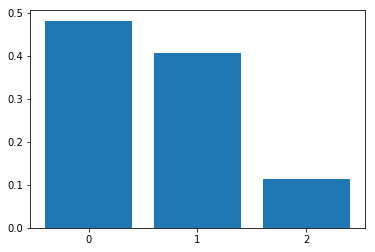
\includegraphics[width=\linewidth]{nn3_damage_90_14_6.png}
			\caption{$ex=6$}
		\end{subfigure}
		\begin{subfigure}{0.33\textwidth}
			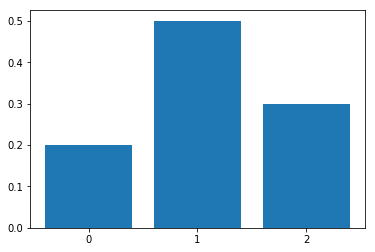
\includegraphics[width=\linewidth]{nn3_damage_90_14_10.png}
			\caption{$ex=10$}
		\end{subfigure}
		\begin{subfigure}{0.33\textwidth}
			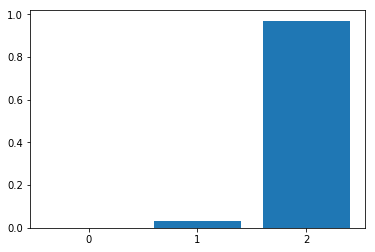
\includegraphics[width=\linewidth]{nn3_damage_90_14_14.png}
			\caption{$ex=14$}
		\end{subfigure}
		\caption{Тест нейросети $nn_{24}$ на балках с повреждениями в $x=90,\ y=14$ и разными $ex$.}
		\label{fig:nn3_damage_90_14}
	\end{figure}

	Результаты, полученные на 10 000-й итерации: \\
	
	\begin{tabular}{| l | l | l | l |}
		\hline
		Нагрузка & Выборка & Потери & Точность \\
		\hline
		2кг & Train & 0.702 & 69.675\% \\
		\hline
		2кг & Test & 0.743 & 69.300\% \\
		\hline
	\end{tabular}
	
	\newpage
	\section{Заключение}
	
	
	В работе был предложен и исследован алгоритм идентификации дефектов при помощи нейронных сетей. Алгоритм был применен к статической задаче с консольной балкой с дефектом.
	
	Были подобраны параметры, при которых алгоритм дал наилучшие результаты. А именно, 2 скрытых слоя по 10 нейронов в каждом, функция активации ReLU, адаптивный градиентный спуск в качестве алгоритма корректировки весов, размер пакета входных данных 64 для задачи поиска местонахождения и 32 для задачи оценки величины повреждения, 10 000 итераций обучения.
	
	Для задачи поиска местонахождения повреждения при его фиксированной величине нейронная сеть была протестирована на балках с разными граничными условиями на правом конце. Точность составила 70.376\% и 69.200\% для нагрузки на правом конце, равной 2кг и 4кг соответственно. То есть, при нагрузке 2кг точность оказалась на 1.176\% выше. Предсказанием нейросети был выбор одного участка балки из 10 возможных. Была рассмотрена также общая задача оценки местонахождения и величины повреждения, при этом предсказанием нейросети для величины повреждения был выбор одного интервала возможных повреждений из 3. В этой задаче нагрузка была взята равной 2кг. Точность составила 61.150\% для местонахождения и 69.300\% для величины повреждения.
	
	\newpage
	\begin{thebibliography}{99}
		
		\bibitem{review}
		Jean-Jacques Sinou,
		A Review of Damage Detection and Health Monitoring of Mechanical Systems from Changes in the Measurement of Linear and Non-linear Vibrations,
		2009.
		
		\bibitem{damage_identification_beam_crossectional_area}
		Dawid Cekus, Mateusz Miara, Izabela Zamorska,
		Damage Identification of a Beam With a Variable Cross-Sectional Area,
		2016.
		
		\bibitem{crack_detection}
		Maged Mostafa, Mohammad Tawfik,
		Crack Detection Using Mixed Axial and Bending Natural Frequencies in Metallic Euler-Bernoulli Beam,
		2016.
		
		\bibitem{artificial_neural_networks_in_damage_detection}
		S. John, A. Kesavan, and I. Herszberg,
		The Use of Artificial Neural Networks in Damage Detection
		and Assessment in Polymeric Composite Structures,
		2010.
		
		\bibitem{randomized_trained_neural_networks}
		Ismoyo Haryanto, Joga Dharma Setiawan, Agus Budiyono,
		Structural Damage Detection Using Randomized Trained Neural Networks,
		2007.
		
		\bibitem{multi_stage_neural_networks}
		Norhisham Bakhary, Hong Hao, Andrew John Deeks,
		Structure Damage Detection Using Neural Network with Multi-Stage Substructuring,
		2010.
		
		\bibitem{imagenet_classification}
		Alex Krizhevsky, Ilya Sutskever, Geoffrey E. Hinton,
		ImageNet Classification with Deep Convolutional Neural Networks.
		
		\bibitem{adagrad}
		John Duchi, Elad Hazan, Yoram Singer, Adaptive Subgradient Methods for Online Learning and Stochastic Optimization, 2011.
		
	\end{thebibliography}

\end{document}